\section{Result Analysis}
\label{sec:ResultAnalysis}

\indent

In this section the results will firstly be analysed and then compared, identifying the differences between the calculated results and the simulation results. The relative differences are calculated according to equation \ref{eq:error}:

\begin{equation}
    e_r = \frac{V_{Octave}-V_{ngspice}}{V_{Octave}} \hspace{5pt}
    \label{eq:error}
\end{equation}

\subsection{Circuit analysis for $t<0$}


\begin{table}[H]
    \caption{Results from the first analysis}
    \begin{subtable}{.5\linewidth}
      \centering
        \caption{Octave}
        \begin{tabular}{ll}
        \hline    
        {\bf Name} & {\bf Value [V]} \\ \hline
        V1 & 5.008942 \\ \hline 
V2 & 4.808960 \\ \hline 
V3 & 4.394159 \\ \hline 
V4 & 0.000000 \\ \hline 
V5 & 4.837862 \\ \hline 
V6 & 5.474755 \\ \hline 
V7 & -2.008723 \\ \hline 
V8 & -2.970917 \\ \hline 

        \end{tabular}
        \begin{tabular}{ll}
        \hline    
        {\bf Name} & {\bf Value [A]} \\ \hline
        Ib & -0.204136 \\ \hline 
Id & 0.000000 \\ \hline 
R1 & 0.194523 \\ \hline 
R2 & -0.204136 \\ \hline 
R3 & -0.009613 \\ \hline 
R4 & 1.156284 \\ \hline 
R5 & 0.204136 \\ \hline 
R6 & 0.961761 \\ \hline 
R7 & 0.961761 \\ \hline 

        \end{tabular}
        \label{tab:OpVOc}
    \end{subtable}%
    \begin{subtable}{.5\linewidth}
      \centering
        \caption{Ngspice}
        \begin{tabular}{ll}
        \hline    
        {\bf Name} & {\bf Value [A or V]} \\ \hline
        @c[i] & 0.000000e+00\\ \hline
@gcs[i] & -2.04136e-04\\ \hline
@r1[i] & 1.945229e-04\\ \hline
@r2[i] & -2.04136e-04\\ \hline
@r3[i] & -9.61363e-06\\ \hline
@r4[i] & 1.156284e-03\\ \hline
@r5[i] & 2.041365e-04\\ \hline
@r6[i] & 9.617613e-04\\ \hline
@r7[i] & 9.617613e-04\\ \hline
v(1) & 5.008942e+00\\ \hline
v(2) & 4.808960e+00\\ \hline
v(3) & 4.394159e+00\\ \hline
v(4) & 0.000000e+00\\ \hline
v(5) & 4.837862e+00\\ \hline
v(6) & 5.474755e+00\\ \hline
v(7) & -2.00872e+00\\ \hline
v(8) & -2.97092e+00\\ \hline

        \end{tabular}
        \label{tab:OpNgs}
    \end{subtable} 
    \label{tab:Op}
\end{table}

The values match almost perfectly. On the table below, the differences are studied with more detail.

\begin{table}[H]
    \caption{Differences on the first analysis}
    \begin{subtable}{.5\linewidth}
      \centering
        \caption{Voltages}
        \begin{tabular}{ll}
        \hline    
        {\bf Name} & {\bf Value [V]} \\ \hline
        \input{../Comparison/Voltages_diff.tex}
        \end{tabular}
        \label{tab:OpVDiff}
    \end{subtable}%
    \begin{subtable}{.5\linewidth}
      \centering
        \caption{Currents}
        \begin{tabular}{ll}
        \hline    
        {\bf Name} & {\bf Value [A]} \\ \hline
        \input{../Comparison/Currents_diff.tex}
        \end{tabular}
        \label{tab:OpCDiff}
    \end{subtable} 
    \label{tab:OpDiff}
\end{table}

This results are commented and explained on the next subsection (subsection \ref{subsection:CAVS}) since they require the same explanation.

\subsection{Circuit analysis for a voltage source-equivalent capacitor}
\label{subsection:CAVS}
\begin{table}[H]
    \caption{Results from the second analysis}
    \begin{subtable}{.5\linewidth}
      \centering
        \caption{Octave}
        \begin{tabular}{ll}
        \hline    
        {\bf Name} & {\bf Value [V]} \\ \hline
        \input{../Analysis/Voltages_2.tex}
        \end{tabular}
        \begin{tabular}{ll}
        \hline    
        {\bf Name} & {\bf Value [A]} \\ \hline
        \input{../Analysis/BranchCurrents_2.tex}
        \end{tabular}
        \label{tab:Op2Oc}
    \end{subtable}%
    \begin{subtable}{.5\linewidth}
      \centering
        \caption{Ngspice}
        \begin{tabular}{ll}
        \hline    
        {\bf Name} & {\bf Value [A or V]} \\ \hline
        @gcs[i] & -2.04136e-04\\ \hline
@r1[i] & 1.945229e-04\\ \hline
@r2[i] & -2.04136e-04\\ \hline
@r3[i] & -9.61363e-06\\ \hline
@r4[i] & 1.156284e-03\\ \hline
@r5[i] & 2.041359e-04\\ \hline
@r6[i] & 9.617613e-04\\ \hline
@r7[i] & 9.617613e-04\\ \hline
v(1) & 5.008942e+00\\ \hline
v(2) & 4.808960e+00\\ \hline
v(3) & 4.394159e+00\\ \hline
v(4) & 0.000000e+00\\ \hline
v(5) & 4.837862e+00\\ \hline
v(6) & 5.474753e+00\\ \hline
v(7) & -2.00872e+00\\ \hline
v(8) & -2.97092e+00\\ \hline

        \end{tabular}
        \label{tab:Op2Ngs}
    \end{subtable} 
    \label{tab:Op2}
\end{table}


\indent

An interesting result appears from this procedure: we notice that the current flows exclusively on the capacitor's mesh (mesh D), on resistor R5. This is explained by the fact that \emph{"current always flows through the path of least resistance"}: since the linearly dependent voltage source has voltage 0 in this instant, it is equivalent to a conductor wire with 0 resistance, configuring a closed circuit with only one resistor (R5). This result appears on table \ref{tab:Op2}.

\begin{table}[H]
    \caption{Differences on the second analysis}
    \begin{subtable}{.5\linewidth}
      \centering
        \caption{Voltages}
        \begin{tabular}{ll}
        \hline    
        {\bf Name} & {\bf Value [V]} \\ \hline
        \input{../Comparison/Voltages_2_diff.tex}
        \end{tabular}
        \label{tab:Op_2VDiff}
    \end{subtable}%
    \begin{subtable}{.5\linewidth}
      \centering
        \caption{Currents}
        \begin{tabular}{ll}
        \hline    
        {\bf Name} & {\bf Value [A]} \\ \hline
        \input{../Comparison/Currents_2_diff.tex}
        \end{tabular}
        \label{tab:Op_2CDiff}
    \end{subtable} 
    \label{tab:Op_2Diff}
\end{table}


The simulation results from both these procedures (table \ref{tab:OpDiff} and \ref{tab:Op_2Diff}) match the predicted ones from the theoretical analysis with great precision (errors are mostly in the range of $10^{-4}\%$). This was expected due to the fact that this circuit only contains linear (dependent and independent) components. The capacitor was not included since it was replaced by a simplified version (an open circuit or a voltage source, respectively).
One detail which is present on both tables is that "\textbf{NaN}" appears on some of the entries. This results from dividing 0 by 0 which happens when the predicted result by \textit{Octave} is 0 and the difference between \textit{Octave} and \textit{Ngspice} is also 0.
Nevertheless, there are very small differences. This could probably originate from numerical approximation on either {\em Octave} or {\em Ngspice} or simulation errors.

\subsection{Circuit analysis for $t>0$}
\subsubsection{Transient analysis: Natural solution}



\begin{figure}[H]
\centering
\begin{subfigure}{.5\textwidth}
  \centering
  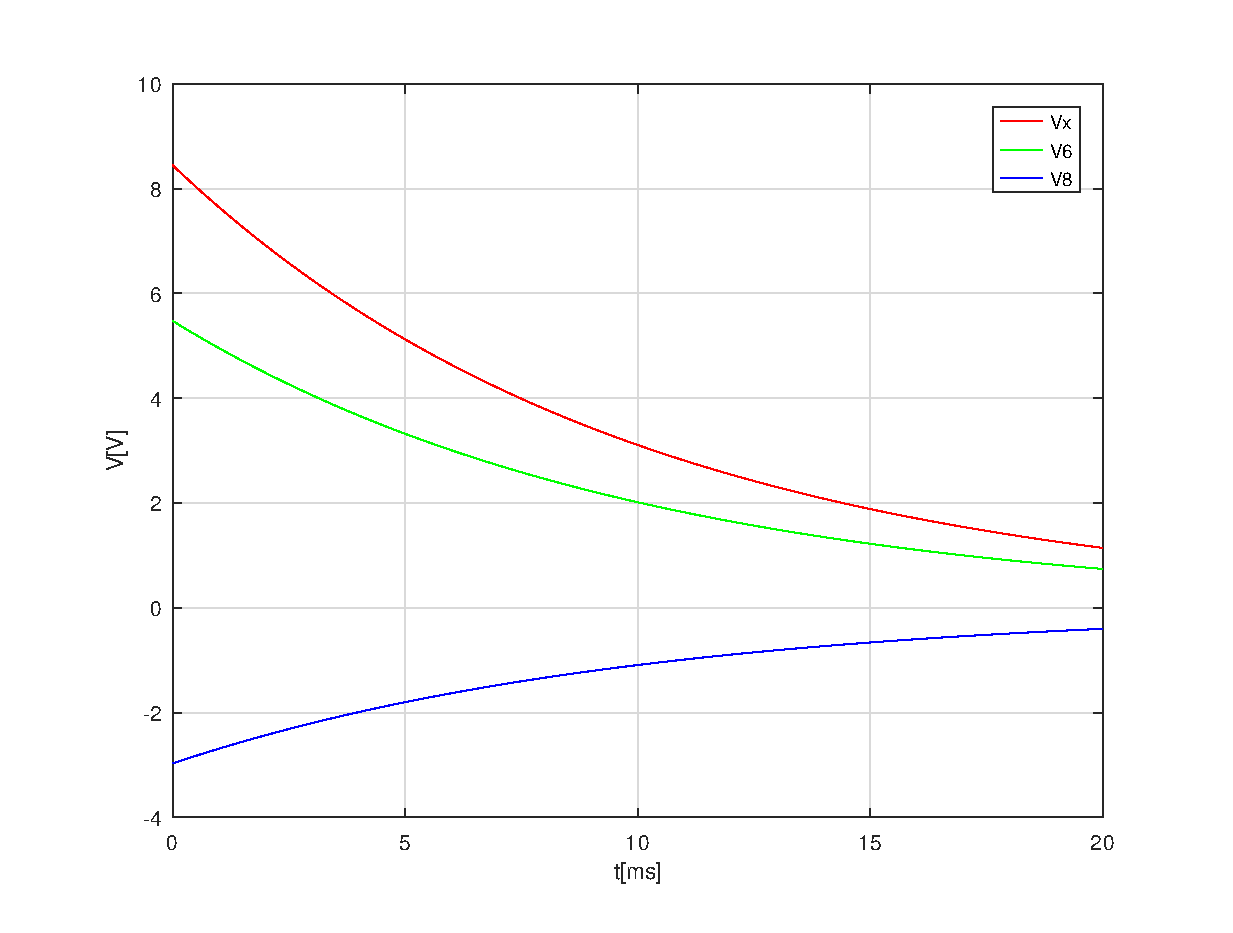
\includegraphics[width=.95\linewidth]{Natural.eps}
  \caption{Octave}
\end{subfigure}%
\begin{subfigure}{.5\textwidth}
  \centering
  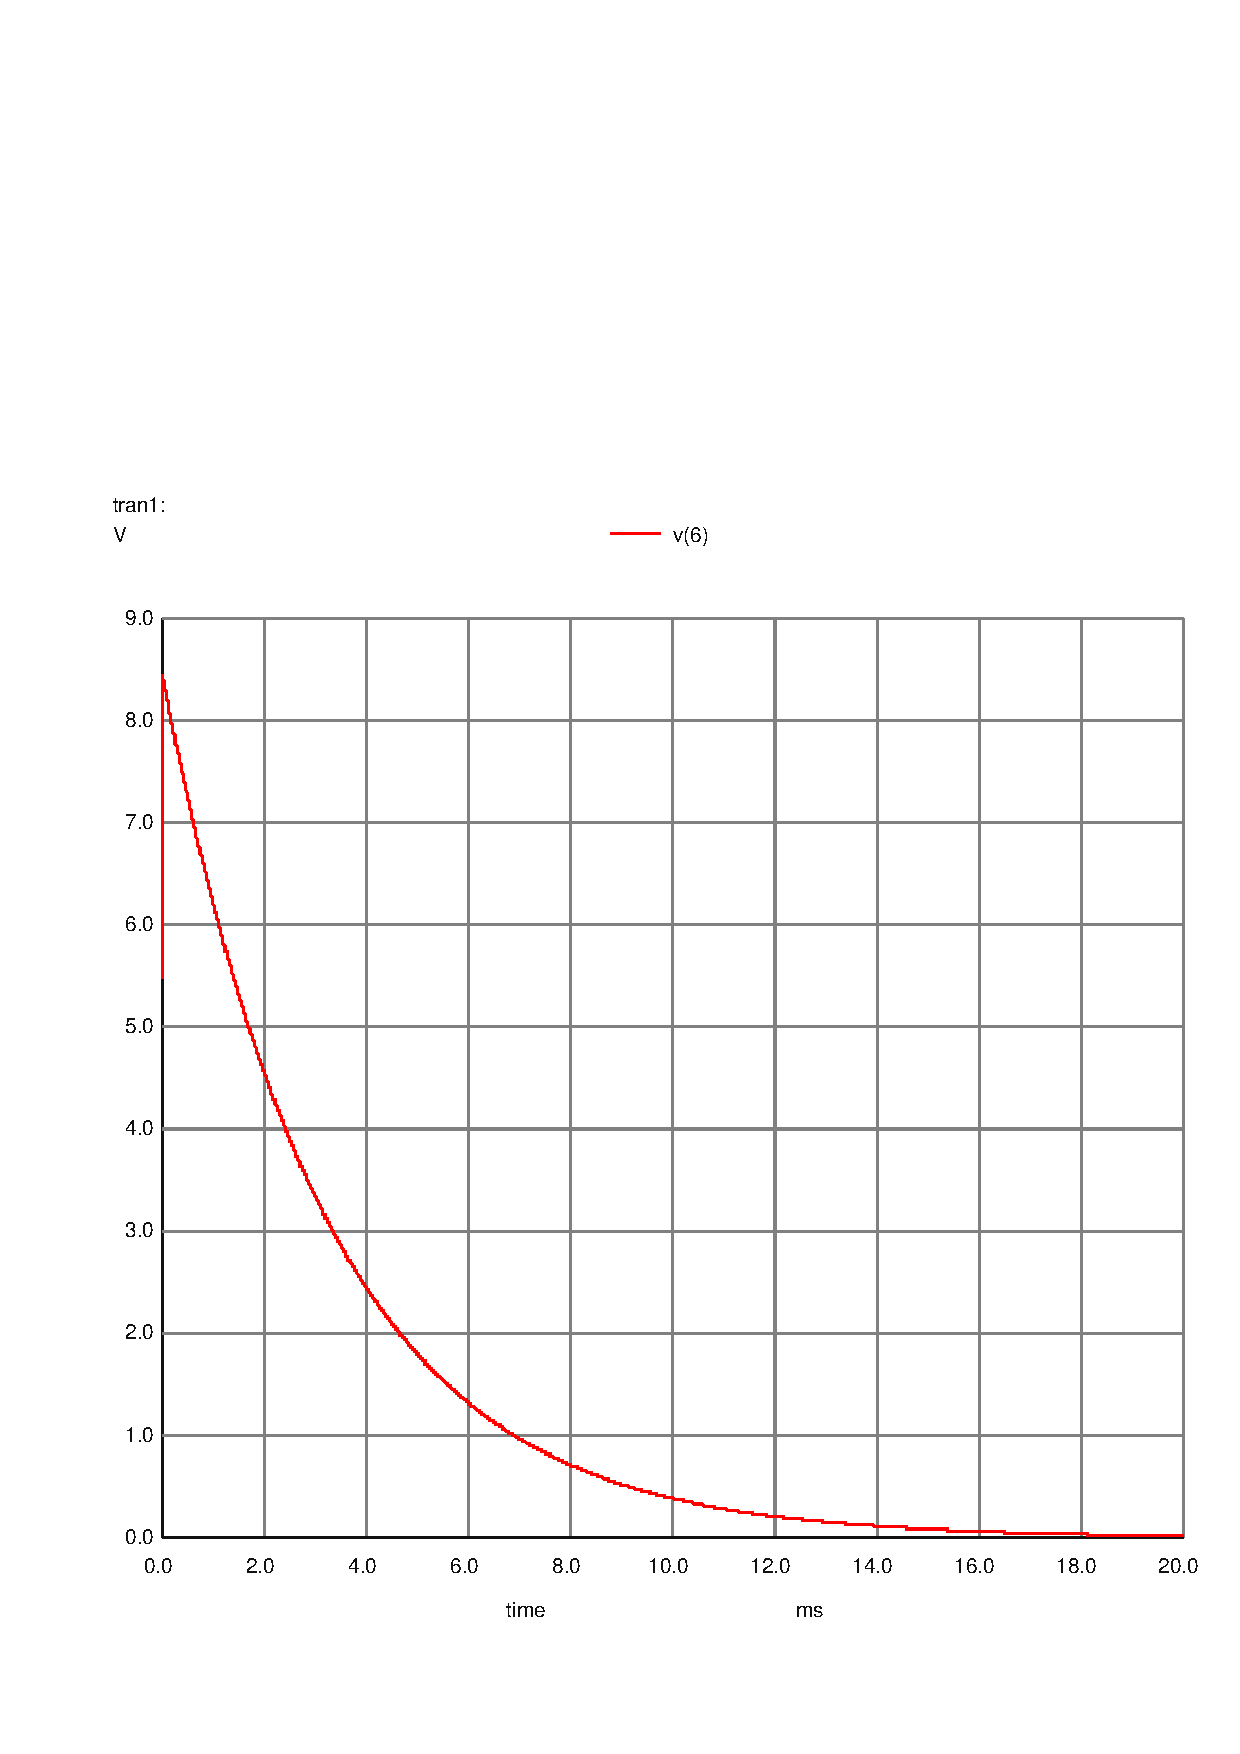
\includegraphics[width=.75\linewidth, trim={2cm 1.5cm 0.5cm 6cm}, clip]{../Simulation/trans_nat.pdf}
  \caption{Ngspice}
\end{subfigure}
\caption{Natural response}
\label{fig:test}
\end{figure}


\indent

As expected the voltages decrease exponentially with time, this represents the capacitor being discharged. Furthermore, it can be seen that the voltage on $V_8$ is zero and that the lines of $V_6$ and $V_x$ are overlapping, meaning the relation $V_x = V_6$ is proved.

\subsubsection{Transient analysis: Final solution}

\indent


\begin{figure}[H]
\centering
\begin{subfigure}{.5\textwidth}
  \centering
  \includegraphics[width=.95\linewidth]{FinalResponse.eps}
  \caption{Octave}
\end{subfigure}%
\begin{subfigure}{.5\textwidth}
  \centering
  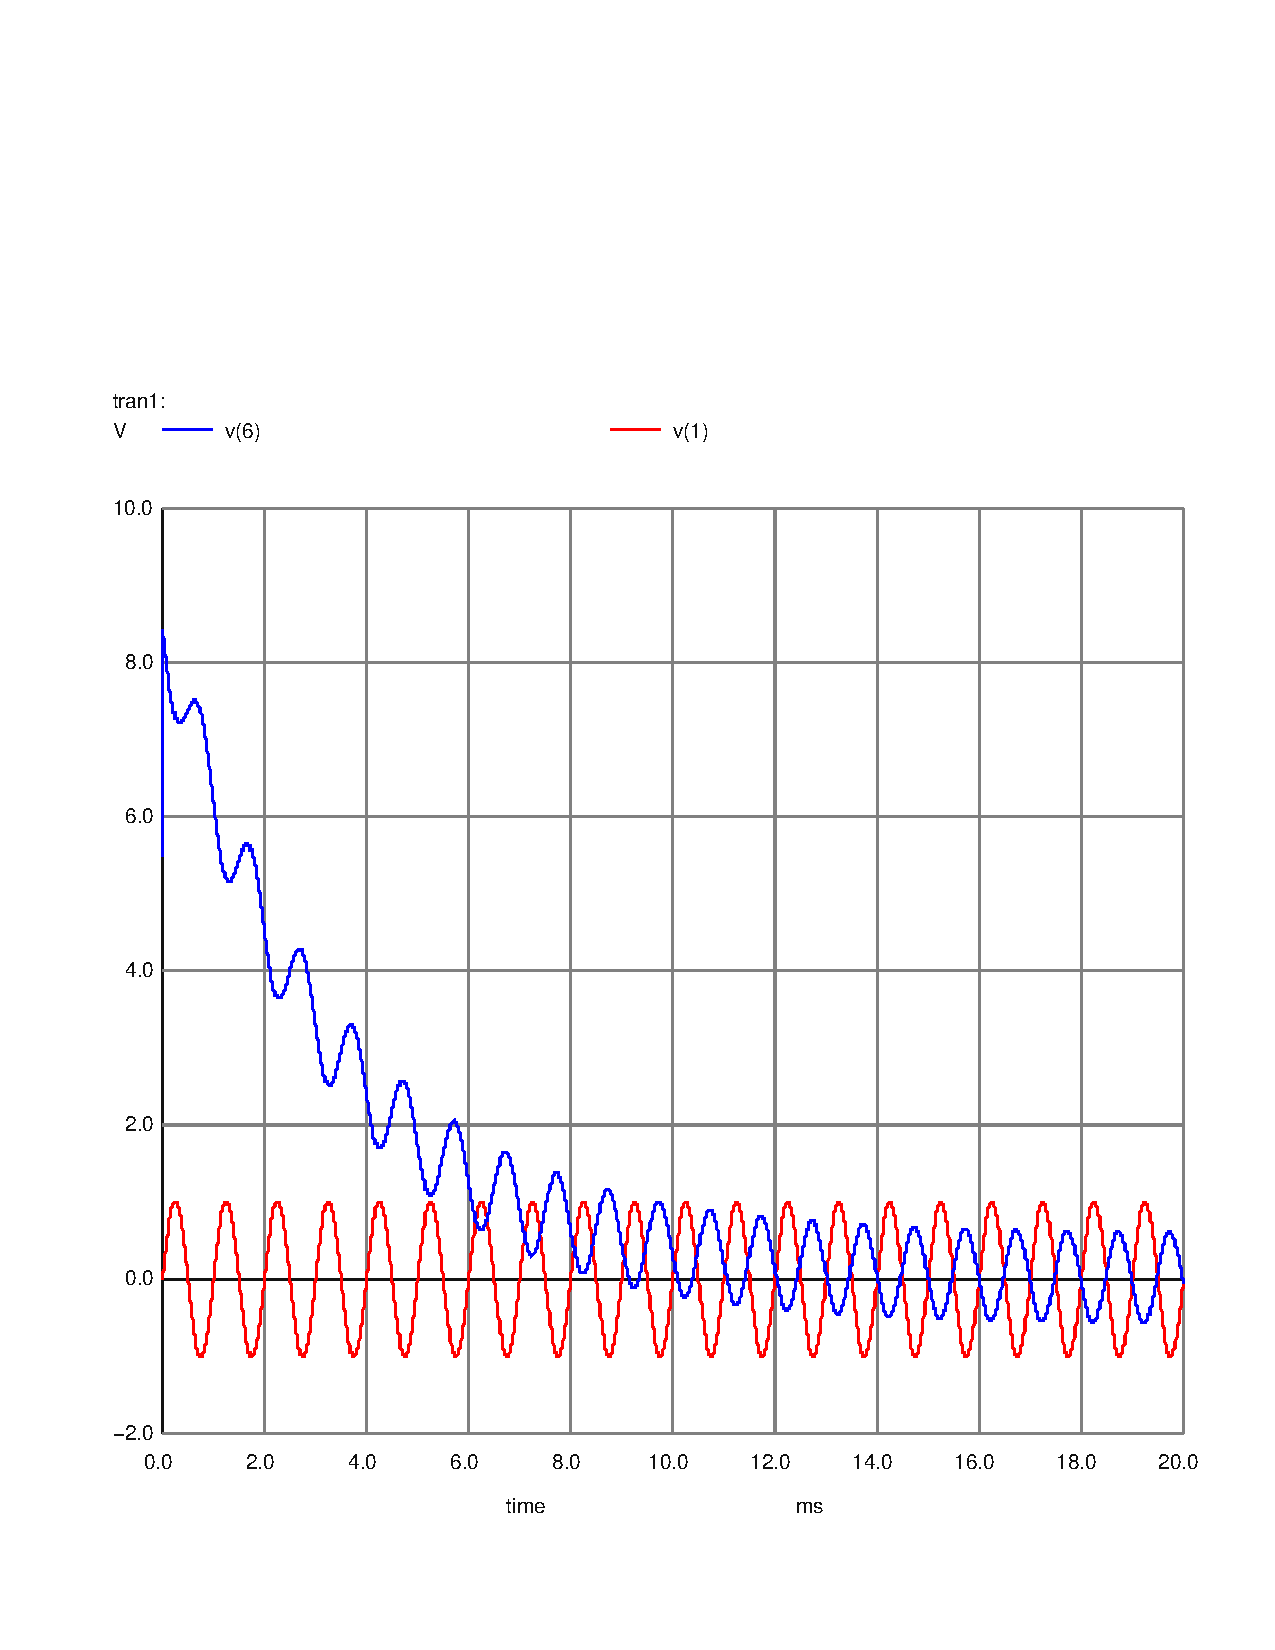
\includegraphics[width=.75\linewidth, trim={2cm 1.5cm 0.5cm 6cm}, clip]{../Simulation/trans_forc.pdf}
  \caption{Ngspice}
\end{subfigure}
\caption{Natural response}
\label{fig:test}
\end{figure}



One aspect that should be mentioned about this data is that the phase of the capacitor is offset to the voltage source by approximately $180^\circ$, and $V_c$ is offset by approximately $90^\circ$. Therefore, its possible to deduce that the current's frequency is greater than the cut-off frequency of this low pass filter (this topic will be further analysed below, on section \ref{sec:Frequency analysis}).
Moreover, $V_x$ decreases with time, approaching zero, but maintains the oscillating regime. This means the capacitor is being discharged until its average is zero. Once this happens the capacitor is lightly charged and discharged in the same frequency as the source.

\subsubsection{Frequency analysis}
\label{sec:Frequency analysis}

\indent



\begin{figure}[H]
\centering
\begin{subfigure}{.5\textwidth}
  \centering
  \includegraphics[width=.95\linewidth]{Magnitude.eps}
  \caption{Octave}
\end{subfigure}%
\begin{subfigure}{.5\textwidth}
  \centering
  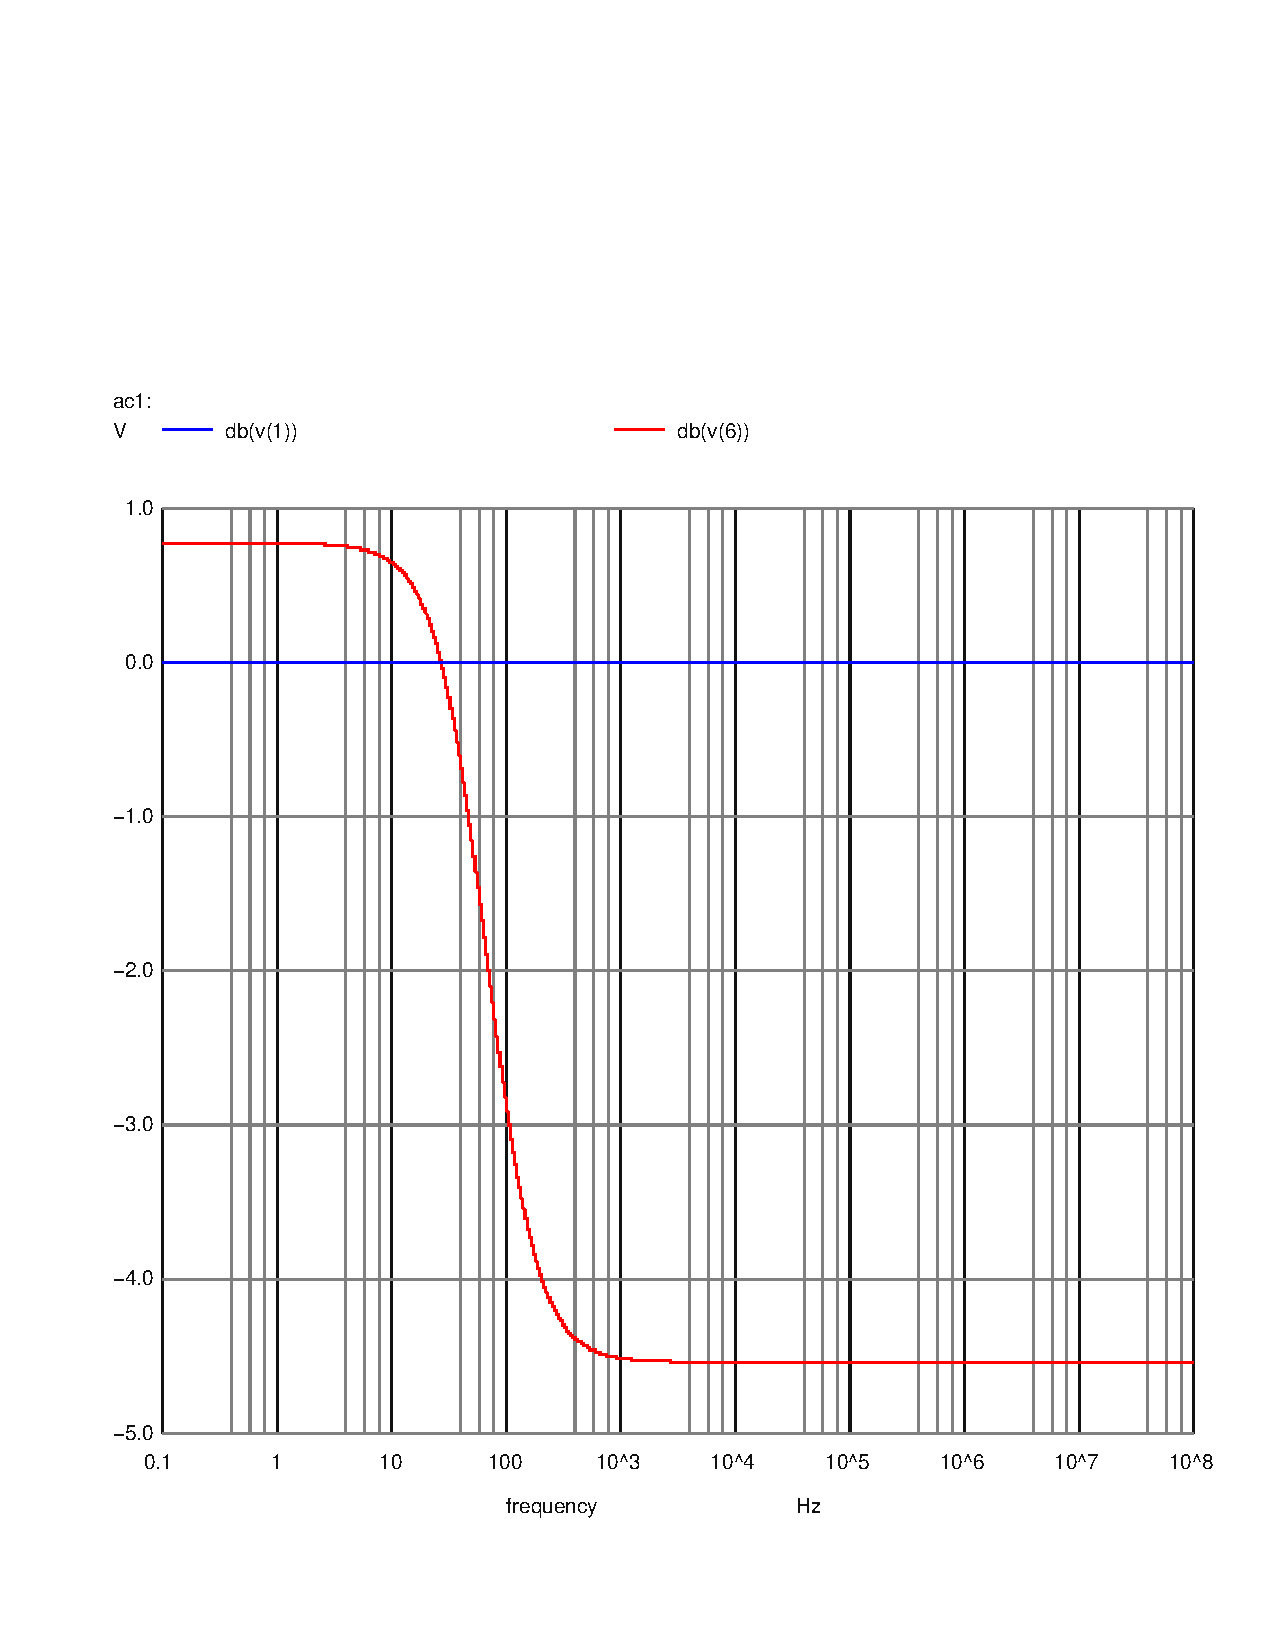
\includegraphics[width=.75\linewidth, trim={2cm 1.5cm 0.5cm 6cm}, clip]{../Simulation/acm_db.pdf}
  \caption{Ngspice}
\end{subfigure}
\caption{Natural response}
\label{fig:test}
\end{figure}



\begin{figure}[H]
\centering
\begin{subfigure}{.5\textwidth}
  \centering
  \includegraphics[width=.95\linewidth]{Phase.eps}
  \caption{Octave}
\end{subfigure}%
\begin{subfigure}{.5\textwidth}
  \centering
  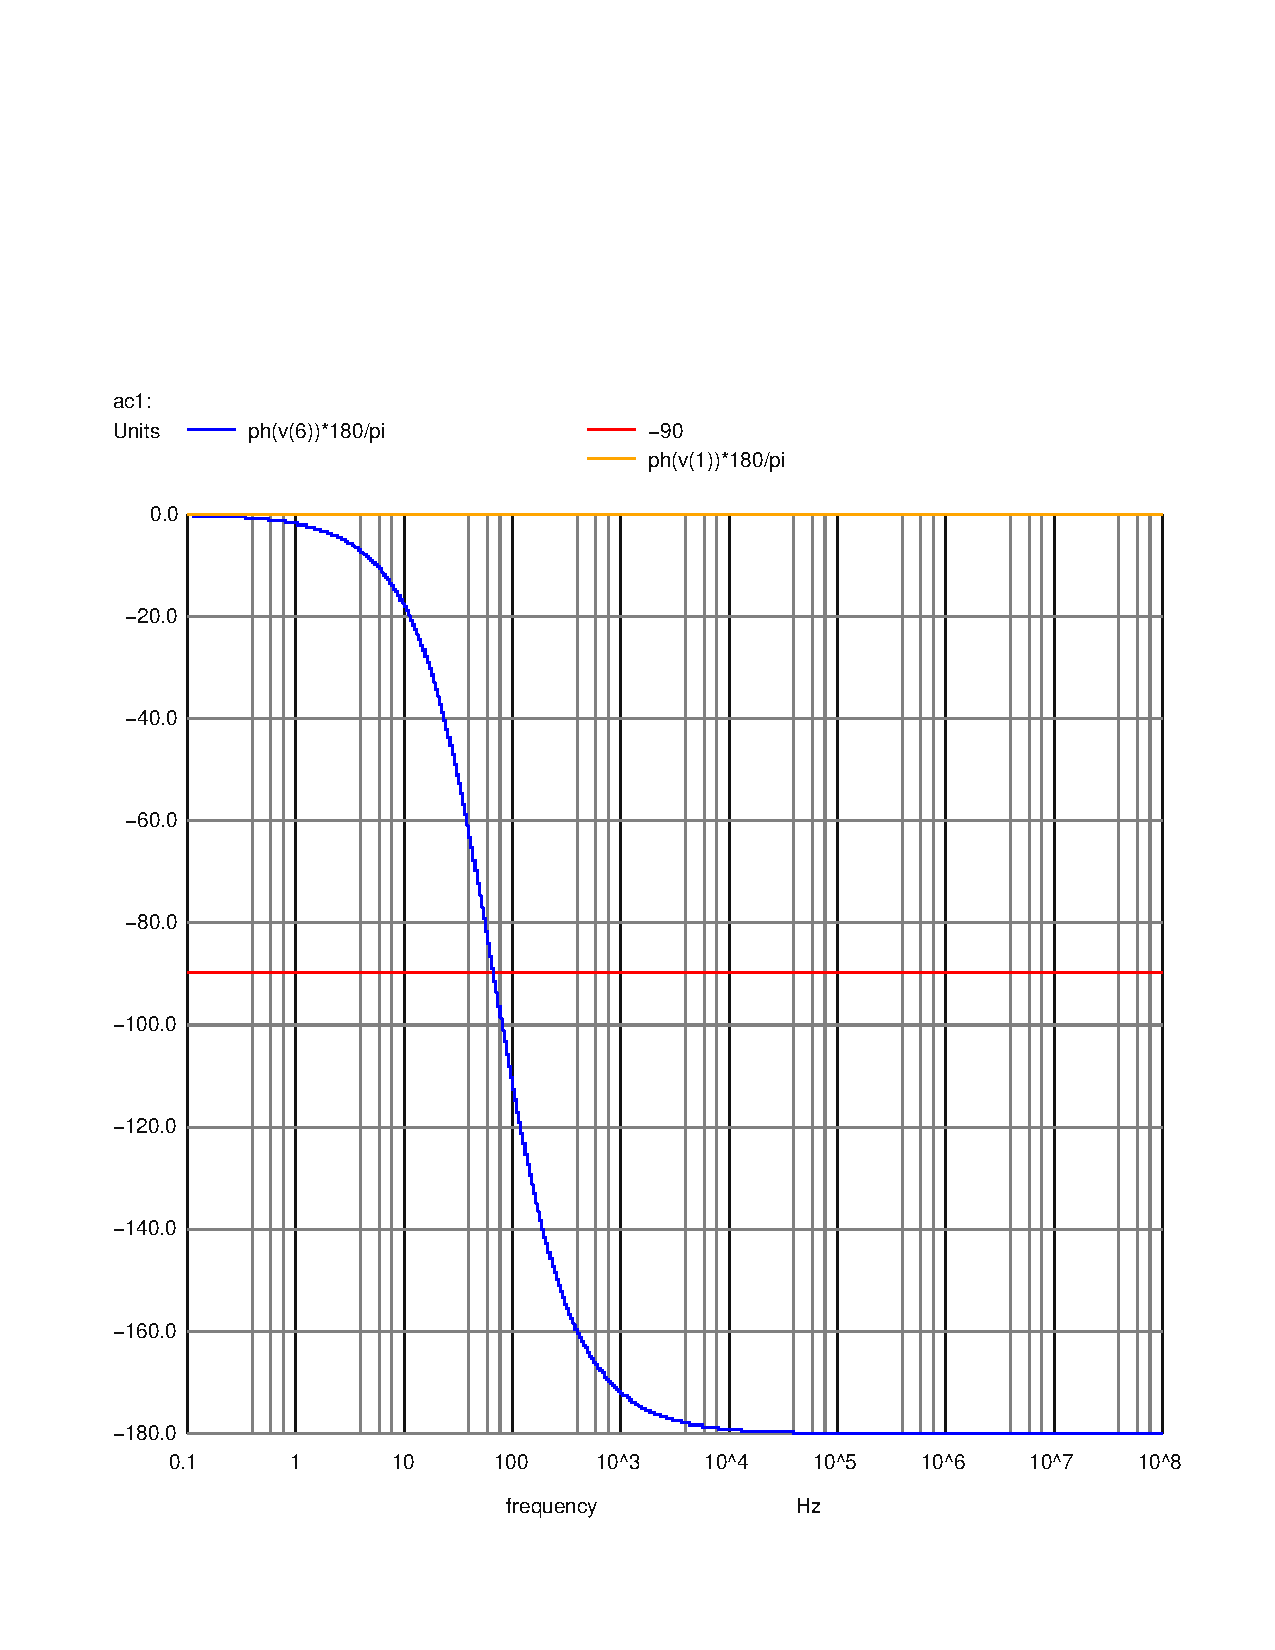
\includegraphics[width=.75\linewidth, trim={2cm 1.5cm 0.5cm 6cm}, clip]{../Simulation/acph.pdf}
  \caption{Ngspice}
\end{subfigure}
\caption{Natural response}
\label{fig:test}
\end{figure}



$V_s$ remains constant since it is the voltage that was taken as the reference (it is an independent voltage source). $V_6$ and $V_c$, on the other hand, have an asymptotic behaviour, tending to offset $-180^\circ$ and $-90^\circ$, respectively.

These graphs confirm that the circuit can be classified as a low-pass filter, since, for low frequencies, the magnitude of voltage on the capacitor ($V_6-V_8$) is close to the one from the voltage source. However this changes on high frequencies, the voltage drops drastically if the frequency increases.

As seen on figure \ref{fig:FreqPhOc}, the cutoff frequency is around $50 Hz$. This value can be confirmed by calculating it according to the equation \ref{eq:cutoff}: \input{../Analysis/Cutoff.tex} Hz. By definition, this frequency is the one with a phase of $45^\circ$.

\begin{equation}
    f_{cutoff} = \frac{1}{2\pi \cdot R_{eq} \cdot C} \hspace{5pt}.
    \label{eq:cutoff}
\end{equation}
